% GNUPLOT: LaTeX picture with Postscript
\begingroup
  \makeatletter
  \providecommand\color[2][]{%
    \GenericError{(gnuplot) \space\space\space\@spaces}{%
      Package color not loaded in conjunction with
      terminal option `colourtext'%
    }{See the gnuplot documentation for explanation.%
    }{Either use 'blacktext' in gnuplot or load the package
      color.sty in LaTeX.}%
    \renewcommand\color[2][]{}%
  }%
  \providecommand\includegraphics[2][]{%
    \GenericError{(gnuplot) \space\space\space\@spaces}{%
      Package graphicx or graphics not loaded%
    }{See the gnuplot documentation for explanation.%
    }{The gnuplot epslatex terminal needs graphicx.sty or graphics.sty.}%
    \renewcommand\includegraphics[2][]{}%
  }%
  \providecommand\rotatebox[2]{#2}%
  \@ifundefined{ifGPcolor}{%
    \newif\ifGPcolor
    \GPcolortrue
  }{}%
  \@ifundefined{ifGPblacktext}{%
    \newif\ifGPblacktext
    \GPblacktexttrue
  }{}%
  % define a \g@addto@macro without @ in the name:
  \let\gplgaddtomacro\g@addto@macro
  % define empty templates for all commands taking text:
  \gdef\gplbacktext{}%
  \gdef\gplfronttext{}%
  \makeatother
  \ifGPblacktext
    % no textcolor at all
    \def\colorrgb#1{}%
    \def\colorgray#1{}%
  \else
    % gray or color?
    \ifGPcolor
      \def\colorrgb#1{\color[rgb]{#1}}%
      \def\colorgray#1{\color[gray]{#1}}%
      \expandafter\def\csname LTw\endcsname{\color{white}}%
      \expandafter\def\csname LTb\endcsname{\color{black}}%
      \expandafter\def\csname LTa\endcsname{\color{black}}%
      \expandafter\def\csname LT0\endcsname{\color[rgb]{1,0,0}}%
      \expandafter\def\csname LT1\endcsname{\color[rgb]{0,1,0}}%
      \expandafter\def\csname LT2\endcsname{\color[rgb]{0,0,1}}%
      \expandafter\def\csname LT3\endcsname{\color[rgb]{1,0,1}}%
      \expandafter\def\csname LT4\endcsname{\color[rgb]{0,1,1}}%
      \expandafter\def\csname LT5\endcsname{\color[rgb]{1,1,0}}%
      \expandafter\def\csname LT6\endcsname{\color[rgb]{0,0,0}}%
      \expandafter\def\csname LT7\endcsname{\color[rgb]{1,0.3,0}}%
      \expandafter\def\csname LT8\endcsname{\color[rgb]{0.5,0.5,0.5}}%
    \else
      % gray
      \def\colorrgb#1{\color{black}}%
      \def\colorgray#1{\color[gray]{#1}}%
      \expandafter\def\csname LTw\endcsname{\color{white}}%
      \expandafter\def\csname LTb\endcsname{\color{black}}%
      \expandafter\def\csname LTa\endcsname{\color{black}}%
      \expandafter\def\csname LT0\endcsname{\color{black}}%
      \expandafter\def\csname LT1\endcsname{\color{black}}%
      \expandafter\def\csname LT2\endcsname{\color{black}}%
      \expandafter\def\csname LT3\endcsname{\color{black}}%
      \expandafter\def\csname LT4\endcsname{\color{black}}%
      \expandafter\def\csname LT5\endcsname{\color{black}}%
      \expandafter\def\csname LT6\endcsname{\color{black}}%
      \expandafter\def\csname LT7\endcsname{\color{black}}%
      \expandafter\def\csname LT8\endcsname{\color{black}}%
    \fi
  \fi
    \setlength{\unitlength}{0.0500bp}%
    \ifx\gptboxheight\undefined%
      \newlength{\gptboxheight}%
      \newlength{\gptboxwidth}%
      \newsavebox{\gptboxtext}%
    \fi%
    \setlength{\fboxrule}{0.5pt}%
    \setlength{\fboxsep}{1pt}%
\begin{picture}(14400.00,5760.00)%
    \gplgaddtomacro\gplbacktext{%
      \csname LTb\endcsname%%
      \put(618,977){\makebox(0,0)[r]{\strut{}\np{e-4}}}%
      \csname LTb\endcsname%%
      \put(618,1742){\makebox(0,0)[r]{\strut{}\np{e-2}}}%
      \csname LTb\endcsname%%
      \put(618,2507){\makebox(0,0)[r]{\strut{}\np{1}}}%
      \csname LTb\endcsname%%
      \put(618,3271){\makebox(0,0)[r]{\strut{}\np{e2}}}%
      \csname LTb\endcsname%%
      \put(618,4036){\makebox(0,0)[r]{\strut{}\np{e4}}}%
      \csname LTb\endcsname%%
      \put(618,4801){\makebox(0,0)[r]{\strut{}\np{e6}}}%
      \csname LTb\endcsname%%
      \put(1147,409){\makebox(0,0){\strut{}\np{e-4}}}%
      \csname LTb\endcsname%%
      \put(2002,409){\makebox(0,0){\strut{}\np{e-2}}}%
      \csname LTb\endcsname%%
      \put(2857,409){\makebox(0,0){\strut{}\np{1}}}%
      \csname LTb\endcsname%%
      \put(3712,409){\makebox(0,0){\strut{}\np{e2}}}%
      \csname LTb\endcsname%%
      \put(4567,409){\makebox(0,0){\strut{}\np{e4}}}%
      \csname LTb\endcsname%%
      \put(5422,409){\makebox(0,0){\strut{}\np{e6}}}%
    }%
    \gplgaddtomacro\gplfronttext{%
      \csname LTb\endcsname%%
      \put(126,2889){\rotatebox{-270}{\makebox(0,0){\strut{}Cross-section (b)}}}%
      \csname LTb\endcsname%%
      \put(3284,130){\makebox(0,0){\strut{}Energy (eV)}}%
      \csname LTb\endcsname%%
      \put(3284,5462){\makebox(0,0){\strut{}Hydrogen \tapi{1}H}}%
      \csname LTb\endcsname%%
      \put(5316,5016){\makebox(0,0)[r]{\strut{}Total}}%
      \csname LTb\endcsname%%
      \put(5316,4830){\makebox(0,0)[r]{\strut{}Elastic}}%
      \csname LTb\endcsname%%
      \put(5316,4644){\makebox(0,0)[r]{\strut{}Capture}}%
    }%
    \gplgaddtomacro\gplbacktext{%
      \csname LTb\endcsname%%
      \put(5748,977){\makebox(0,0)[r]{\strut{}}}%
      \csname LTb\endcsname%%
      \put(5748,1742){\makebox(0,0)[r]{\strut{}}}%
      \csname LTb\endcsname%%
      \put(5748,2507){\makebox(0,0)[r]{\strut{}}}%
      \csname LTb\endcsname%%
      \put(5748,3271){\makebox(0,0)[r]{\strut{}}}%
      \csname LTb\endcsname%%
      \put(5748,4036){\makebox(0,0)[r]{\strut{}}}%
      \csname LTb\endcsname%%
      \put(5748,4801){\makebox(0,0)[r]{\strut{}}}%
      \csname LTb\endcsname%%
      \put(5850,409){\makebox(0,0){\strut{}\np{e-5}}}%
      \csname LTb\endcsname%%
      \put(6502,409){\makebox(0,0){\strut{}\np{e-4}}}%
      \csname LTb\endcsname%%
      \put(7155,409){\makebox(0,0){\strut{}\np{e-3}}}%
      \csname LTb\endcsname%%
      \put(7807,409){\makebox(0,0){\strut{}\np{e-2}}}%
      \csname LTb\endcsname%%
      \put(8460,409){\makebox(0,0){\strut{}\np{0.1}}}%
      \csname LTb\endcsname%%
      \put(9112,409){\makebox(0,0){\strut{}\np{1}}}%
      \csname LTb\endcsname%%
      \put(9765,409){\makebox(0,0){\strut{}\np{10}}}%
      \csname LTb\endcsname%%
      \put(10417,409){\makebox(0,0){\strut{}\np{e2}}}%
      \csname LTb\endcsname%%
      \put(11069,409){\makebox(0,0){\strut{}\np{e3}}}%
      \csname LTb\endcsname%%
      \put(11722,409){\makebox(0,0){\strut{}\np{e4}}}%
      \csname LTb\endcsname%%
      \put(12374,409){\makebox(0,0){\strut{}\np{e5}}}%
      \csname LTb\endcsname%%
      \put(13027,409){\makebox(0,0){\strut{}\np{e6}}}%
      \csname LTb\endcsname%%
      \put(13679,409){\makebox(0,0){\strut{}\np{e7}}}%
    }%
    \gplgaddtomacro\gplfronttext{%
      \csname LTb\endcsname%%
      \put(5748,2889){\rotatebox{-270}{\makebox(0,0){\strut{}}}}%
      \csname LTb\endcsname%%
      \put(9764,130){\makebox(0,0){\strut{}Energy (eV)}}%
      \csname LTb\endcsname%%
      \put(9764,5462){\makebox(0,0){\strut{}Gadolinium \tapi{155}Gd}}%
      \csname LTb\endcsname%%
      \put(13146,5016){\makebox(0,0)[r]{\strut{}Total}}%
      \csname LTb\endcsname%%
      \put(13146,4830){\makebox(0,0)[r]{\strut{}Elastic}}%
      \csname LTb\endcsname%%
      \put(13146,4644){\makebox(0,0)[r]{\strut{}Capture}}%
    }%
    \gplgaddtomacro\gplbacktext{%
      \csname LTb\endcsname%%
      \put(8660,720){\makebox(0,0)[l]{\strut{}\np{1}}}%
      \csname LTb\endcsname%%
      \put(8660,1872){\makebox(0,0)[l]{\strut{}\np{e2}}}%
      \csname LTb\endcsname%%
      \put(8660,3023){\makebox(0,0)[l]{\strut{}\np{e4}}}%
      \csname LTb\endcsname%%
      \put(7786,3209){\makebox(0,0){\strut{}\np{50}}}%
      \csname LTb\endcsname%%
      \put(5994,3209){\makebox(0,0){\strut{}\np{10}}}%
      \csname LTb\endcsname%%
      \put(8558,3209){\makebox(0,0){\strut{}\np{e2}}}%
    }%
    \gplgaddtomacro\gplfronttext{%
      \csname LTb\endcsname%%
      \put(6003,1871){\rotatebox{-270}{\makebox(0,0){\strut{}}}}%
      \csname LTb\endcsname%%
      \put(7276,664){\makebox(0,0){\strut{}}}%
      \csname LTb\endcsname%%
      \put(7276,3116){\makebox(0,0){\strut{}}}%
    }%
    \gplbacktext
    \put(0,0){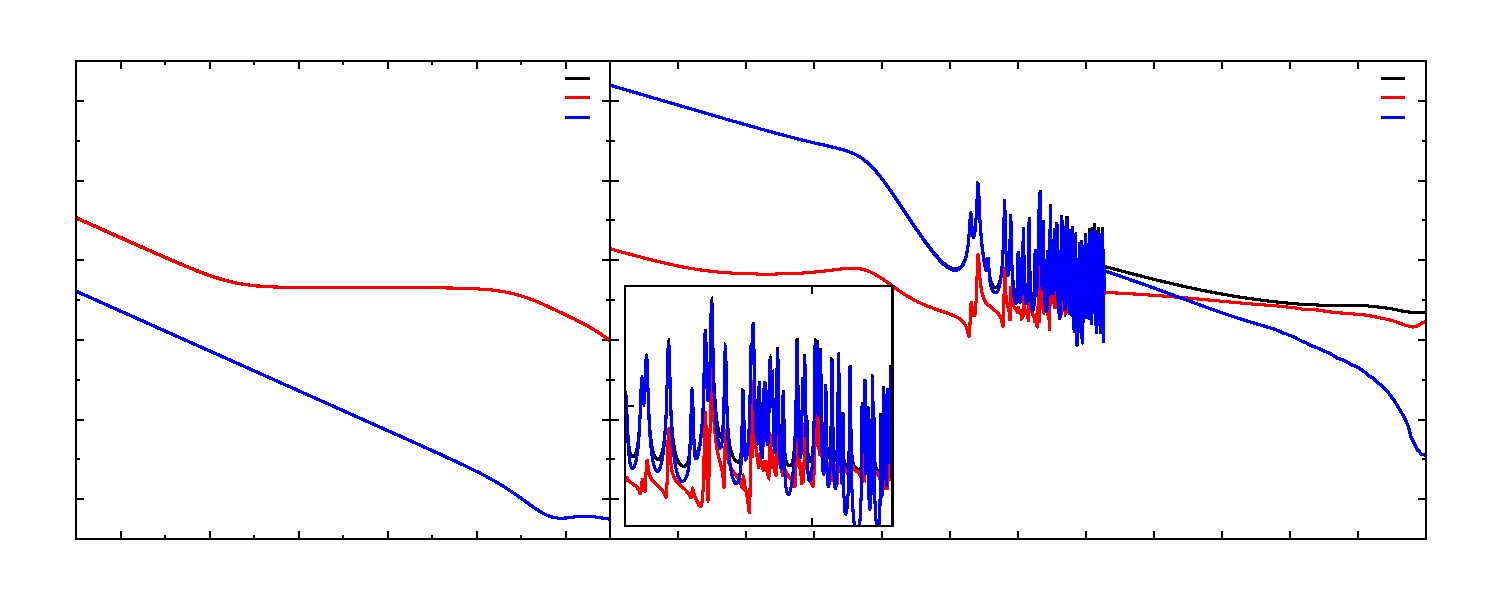
\includegraphics{neutron_xsec}}%
    \gplfronttext
  \end{picture}%
\endgroup
